\chapter{多方参与业务下的隐私保护模型}
为了满足去中心化计算的特质似乎存在一个潜在的要求,即智能合约的执行逻辑与输入输出数据对于所有节点来说都是透明的。而这一约束极大限制了存在数据隐私需求的应用实现去中心化特性。

有助于解除这一约束的密码学工具是零知识证明技术。如前所述,研究人员已经提出了一些满足各种隐私定义与信任假设的系统\cite{7546538, 2018arXiv180405141C}。然而这些工作并没有讨论到针对多方参与业务下的适用性。他们对系统的具现化实现和对特定信任的强依赖使得模型通常只能工作在特定场景中而不能满足各类应用的开发需求。对此,我们尝试通过本章解答这一问题:\textbf{在多方参与业务下是否存在一个满足去中心化特性的隐私保护智能合约模型?}

\section{模型架构}
在本节我们将对系统中涉及的模块进行介绍与功能划分,这有助于我们后续对系统拆分进行单独建模并组合为一个通用模型。
\subsection{基础结构}
\begin{figure}[htbp]
    \centering
    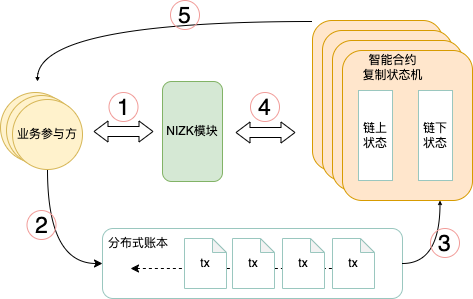
\includegraphics[width=.7\linewidth]{ch3/ch3-2}
    \caption{\label{fig:ch3-structure}模型架构图}
\end{figure}

\paragraph{智能合约} 尽管在隐私保护的系统模型中为了实现对数据与计算逻辑的保护,智能合约的行为变得更为复杂,然而其实质上每次智能合约的调用过程的都是一次账本状态由旧到新的变更。因此为了简化复杂合约行为与账本的交互,我们将协同计算模型中的智能合约建模为复制状态机。实际系统中的交易请求,对应在模型中状态机的输入即为一些固定语义的高级命令。

值得一提的是在通用的协同计算模型下的智能合约可以被细化为两个部分,即链上合约与链下合约,分别维护了分布式账本上公共状态$\sigma$和链下节点的私有状态。对于链下节点$\mathit{p}$,对应的私有状态记为$\rho_\mathit{p}$。对于某个链下计算节点$p$来说,对应的智能合约状态可以描述为$(\sigma, \rho_\mathit{p})$。虽然诚实的链下计算节点,往往根据预先约定的合约行为更新自己的私有状态。但是合约设计者必须意识到链下节点的私有状态更新是不被默认信任的,不诚实节点可以随意更改他们的状态。因此我们加入了计算证明来保证链下计算的正确性和可信性,当然这也增加了交互代价和链上存储的大小。

\paragraph{分布式账本} 基于上述职能合约的设计,区块链对应的分布式账本系统可以被更为简单的表示为交易记录模型。即在模型中分布式账本实际上维护了一个交易序列,任何参与方都可以向其提交新的交易,一旦交易被记录在序列中,所有参与方都可以查看最新的交易序列及交易的全部内容。为了简化模型,在这里我们省略了链上交易的排序共识模块,从而默认账本能够按照正确顺序记录交易序列。

\paragraph{NIZK证明} 根据之前的研究综述,我们发现非交互式的零知识证明(NIZK)是链下计算技术的一个理想实现方案。因此整体的隐私保护模型构建时,我们基于这一方案进行阐述。在整个模型中,需要调用NIZK模块作计算的证明和链上的验证,其中证明发生在业务参与方对应的链下计算节点进行链下计算生成交易的过程中,验证则发生在合约状态更新的过程中。

\subsection{功能定义}
我们将触发一次协同计算业务执行的全过程,即$(\sigma, \rho_\mathit{p})\rightarrow(\sigma', \rho_\mathit{p}')$,定义为协同计算中的一个中间段。则对于一次涉及$n$次状态变更的完整的协同计算$(\sigma, \rho)\rightarrow(\sigma^n, \rho_{p_0,\dots,p_n})$可以拆分为$(\sigma, \rho)\rightarrow(\sigma^0, \rho_{p_0})\rightarrow(\sigma^1, \rho_{p_0,p_1})\rightarrow \dots \rightarrow (\sigma^n, \rho_{p_0,\dots,p_n})$。这一定义有助于我们简化一些复杂的业务合约行为,例如一笔交易引发的链上链下协同计算执行过程中包含多方链下隐私计算。

基于\autoref{fig:ch3-structure}构建的模型示意图,我们可以简单描述出一次的完整的隐私保护业务计算过程。如下所述,在一次计算过程中,智能合约触发的链下计算请求成为两次状态变更的桥梁。
\begin{enumerate}
    \setlength{\itemsep}{0pt}
    \setlength{\parsep}{0pt}
    \setlength{\parskip}{0pt}
\item 业务参与方$p$构建一笔包含链下计算证明的业务交易提交给分布式账本。
\item 智能合约按照账本中的交易顺序依次执行,在该过程中将调用NIZK模块验证内容的合法性。
\item 若交易合法则更新合约状态$(\sigma, \rho_p)$,否则跳过该交易。
\item 对于合法交易返回执行结果,并且根据业务逻辑发起新的链下计算的调用请求$\mathit{q}$到其他业务参与方$p$;若不存在新的链下计算调用,则业务执行完成,通知业务发起方。
\item 对于收到请求的业务方继续按照步骤1执行。
\end{enumerate}

但需要注意的是,在业务参与方对应链下计算节点并发处理多次链下计算请求时,我们必须考虑计算的执行顺序。一组计算在不同的执行顺序下可能出现不同的状态更新结果。在第四章中,我们将对这些情况作深入分析。
\section{协同计算下的智能合约模型}
智能合约通常被描述并实现为复制状态机,传递给状态机的输入一般从记录在账本上的交易中获取。为了描述隐私保护的智能合约模型,我们需要对这一定义作调整。这是因为如果所有输入都来自分布式账本上的交易,其无法有效表示合约中针对链下计算及其隐私输入完成的状态变化。在由链下计算节点发起的包含链下计算的状态转移过程中由于NIZK模块的作用,并不能根据交易内容中的证明直接得到链下隐私状态。对此,我们将传递给状态机的输入替换为生成交易时提供的所有输入。此外基于模型设计,我们的智能合约中需要包含对后续参与方链下计算请求的调用,因此执行结果在计算输出之外还应包含对链下计算的请求集合$Q$。我们给出智能合约的整体状态转移函数如下:
\begin{center}
    $\Gamma:(\phi', c, y, Q) \leftarrow f(\phi, p, w)$
\end{center}
其中,$\phi$表示合约初始状态;$\phi'$表示合约执行后的新状态;$p$为链下计算方;$w$为创建交易时给定的输入;$y$为执行返回结果;$c$代表是否成功执行。

如\autoref{fig:ch3-structure}所示,基于隐私保护的智能合约状态应包含两部分:链上与链下。状态的转移依赖于对链下计算证明的验证过程,因此我们将对上述转移函数作进一步细化,将其分为链上合约和链下合约两部分从而方便与后续的证明模块相匹配。我们首先对单部分的合约执行过程作建模,随后将其扩展为链上链下两个合约模块。

\subsection{合约执行模型}
与KACHAIN\cite{9505181}类似,我们将执行过程定义为一组对状态变更的请求记录。将合约状态看作一个交互式的模块,则整个合约执行过程可以被看作由基于外界输入生成的固定交互请求集合构成。每次交互都是申请对合约状态的修改,如果修改成功则返回结果,如果失败则返回$\perp$。那么对于维护着状态$\alpha$的合约状态执行模型$\mathcal{O}_\alpha$来说,其允许的交互方式可以定义为:
\begin{breakablealgorithm}
    \caption{合约执行模型$\mathcal{O}_{\alpha}$}
    \label{alg:ch3-1}
    \begin{algorithmic} 
    \item [初始状态]:
    \STATE let $\mathcal{T} \leftarrow \epsilon$
    \item [收到请求$q$]:
    \STATE 计算$(\alpha, r) \leftarrow q(\alpha)$
    \IF {$\alpha = \perp$}
    \STATE $r = \perp$
    \ENDIF
    \STATE $\mathcal{T} \leftarrow \mathcal{T} \parallel (q, r)$
    \STATE return $r$
    \item [$check(\mathcal{O}_{\alpha})$]:
    \STATE return $\alpha, \mathcal{T}$
    \end{algorithmic}
\end{breakablealgorithm}

如\autoref{fig:ch3-transfer}所示,则对于输入$w$来说,其基于合约状态$\mathcal{O}_{\alpha}$的执行结果可以表示为$(y, Q) \leftarrow f_{\mathcal{O}_\alpha}(w)$,而相应的合约状态转移为$\alpha \leftarrow \mathcal{T}_\alpha(\alpha)$。其中,
\begin{center}
    $\mathcal{O}_{\alpha} \leftarrow (\alpha)$ \newline
    $(\alpha, \mathcal{T}_\alpha) \leftarrow check(\mathcal{O}_{\alpha}), \mathcal{T}_\alpha: \{(q_1, r_1), (q_2, r_2), \dots, (q_i, r_i)\}$
\end{center}
\begin{figure}[htbp]
    \centering
    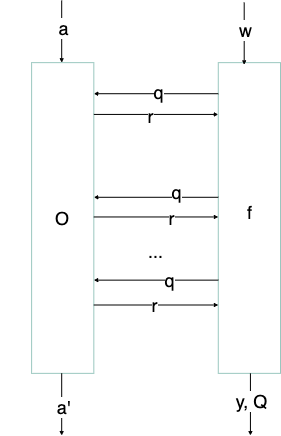
\includegraphics[width=.3\linewidth]{ch3/ch3-3}
    \caption{\label{fig:ch3-transfer}智能合约状态交互图}
\end{figure}
\subsection{状态转移函数}
综上,将其扩展至协同计算中可以其交互如图\autoref{fig:ch3-offchain}所示。对原本的状态转移函数进行细化,其内部的执行逻辑可以表示为:
\begin{breakablealgorithm}
    \caption{状态转移函数$\Gamma$}
    \label{alg:ch3-2}
    \begin{algorithmic} 
        \item [$((\sigma, \rho), c, y, Q) \leftarrow \Gamma((\sigma, \rho), p, w)$]
        \STATE let $c \leftarrow \perp$
        \STATE let $(\mathcal{T}_\sigma, \mathcal{T}_\rho, y, Q) \leftarrow \Gamma_{mid}((\sigma, \rho), p, w)$
        \STATE let $\sigma' = \mathcal{T}_\sigma(\sigma), \rho' = \mathcal{T}_\rho(\rho)$
        \IF {$\sigma' \neq \perp \wedge \rho' \neq \perp$}
        \STATE $c \leftarrow \top, (\sigma, \rho) \leftarrow (\sigma', \rho')$
        \ENDIF
        \STATE return $((\sigma, \rho), c, y, Q)$

        \noindent\hrulefill
        \item [$(\mathcal{T}_\sigma, \mathcal{T}_\rho, y, Q) \leftarrow \Gamma_{mid}((\sigma, \rho), p, w)$]:
        \STATE let $\mathcal{O}_{\rho} \leftarrow \rho, \mathcal{O}_{\sigma} \leftarrow \sigma, (y, Q) \leftarrow f_{\mathcal{O}_\sigma, \mathcal{O}_\rho}(w)$
        \STATE let $(\sigma', \mathcal{T}_\sigma) \leftarrow check(\mathcal{O}_\sigma), (\rho', \mathcal{T}_\rho) \leftarrow check(\mathcal{O}_\rho)$
        \STATE return $(\mathcal{T}_\sigma, \mathcal{T}_\rho, y, Q)$
    \end{algorithmic}
\end{breakablealgorithm}
\begin{figure}[htbp]
    \centering
    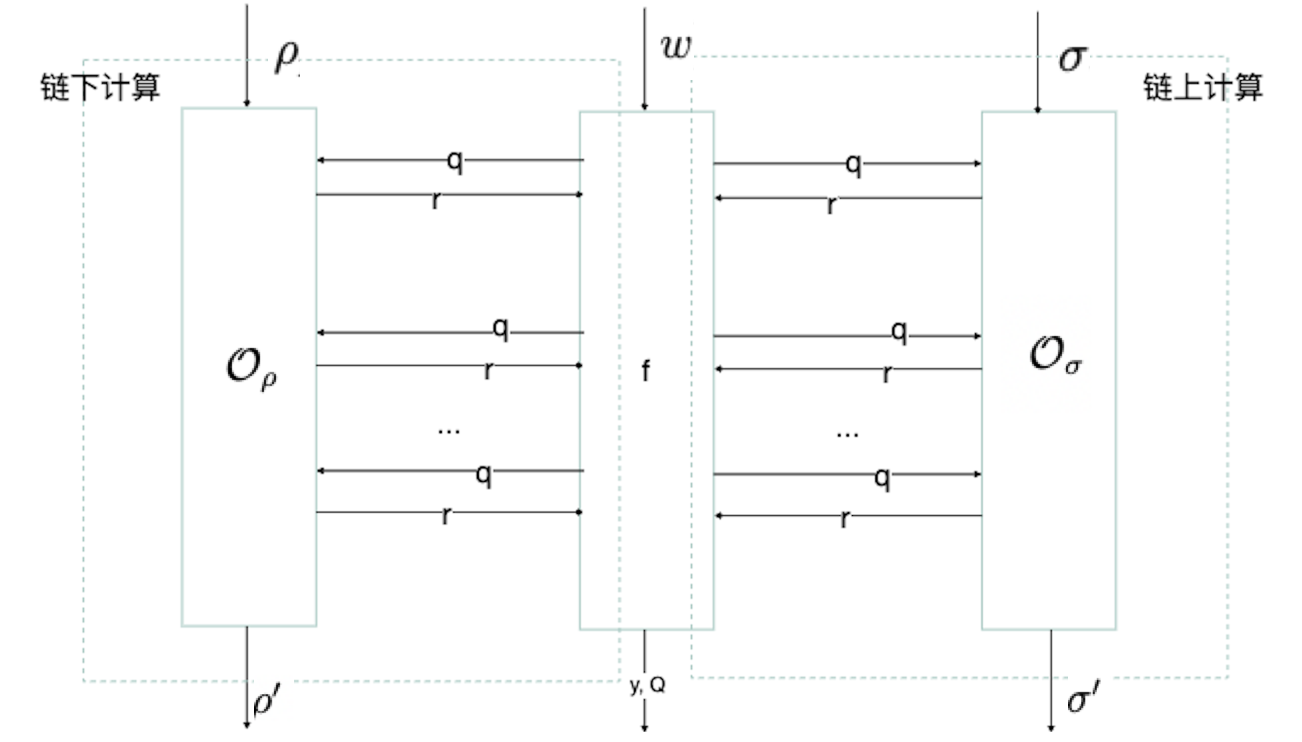
\includegraphics[width=.8\linewidth]{ch3/ch3-4}
    \caption{\label{fig:ch3-offchain}协同计算状态交互图}
\end{figure}

\section{协同计算下的NIZK模型}
NIZK模块主要负责完成对链下计算过程生成NIZK证明以及提供NIZK验证,是隐私保护的协同计算过程中不可或缺的部分。虽然很多基于零知识证明技术的工作都包含了对隐私计算的实现设计,然而很少有工作基于协同计算对其进行抽象化的描述。本节中,我们首先对NIZK的算法定义作介绍,随后将其在协同计算模型中的功能使用函数的形式表示出来。

\subsection{NIZK相关定义}
一个NIZK协议有两个参与者,即证明方P与验证方V,P希望说服V相信其拥有证明某个命题(statement)成立的知识(witness),整个过程需要满足以下几个特性:
\begin{itemize}
    \setlength{\itemsep}{0pt}
    \setlength{\parsep}{0pt}
    \setlength{\parskip}{0pt}
\item 完整性:证明者拥有使命题成立的witness的能通过验证,也就是在statement为真时可通过验证
\item 可靠性:恶意的证明者在陈述为假时无法通过验证
\item 零知识:V将无法得到除statement真假之外的其他信息,即证明和验证过程能够在不透露witness的情况下进行
\item 非交互性:不需要P与V之间的多轮交互
\end{itemize}

\subsection{协同计算下的NIZK描述}
在协同计算中的链下计算过程并不可信,因此我们需要对链下计算生成证明$\pi$,在验证其合法性后才可以将应用链下状态。如\autoref{fig:ch3-offchain}所示,基于3.2中的状态转移模型,我们可以把链上状态转移与链下划分开来。对于以$\mathcal{T}_\sigma$代表的链上状态交互序列是公开可验证的,而$\mathcal{T}_\rho$的部分则为链下隐私计算中发生的。

因此我们可以将$\mathcal{T}_\sigma$作为NIZK的公开输入,而其链下的计算$\mathcal{T}_\rho$就作为witness,从而构建对于协同计算的statement:收到输入$w$后,链上计算与链下计算对应的状态变更步骤集合分别为$\mathcal{T}_\sigma, \mathcal{T}_\rho$。当执行后的状态不为$\perp$时,才能将$\mathcal{T}_\sigma, \mathcal{T}_\rho$应用到账本中。其对应的公式描述为:
\begin{center}
    $(\mathcal{T}_\sigma, \mathcal{T}_\rho) \in \mathcal{L}:$ \newline $\mathcal{O}_\sigma \leftarrow \mathcal{O}(\mathcal{T}_\sigma), \mathcal{O}_\rho \leftarrow \mathcal{O}(\mathcal{T}_\rho), (\sigma', \cdot) \leftarrow check(\mathcal{O}_\sigma), (\rho', \cdot) \leftarrow check(\mathcal{O}_\rho), \sigma' \neq \perp \wedge \rho' \neq \perp$
\end{center}

协同计算中创建NIZK证明与验证的过程如下所示,我们用$\Pi$指代已创建的公开输入与证明的配对关系。其中$NIZK$方法用于使用具体NIZK算法生成证明。

\begin{breakablealgorithm}
    \caption{协同计算中的NIZK模型$\mathcal{F}_{NIZK}$}
    \label{alg:ch3-3}
    \begin{algorithmic} 
        \item [初始状态]: $\Pi \leftarrow \epsilon$
        \item [收到证明请求]: $PROVE(\mathcal{T}_\sigma, \mathcal{T}_\rho)$
        \IF {$(\mathcal{T}_\sigma, \mathcal{T}_\rho) \notin \mathcal{L}$}
        \STATE return $\perp$
        \ENDIF
        \STATE $\pi \leftarrow NIZK(\mathcal{T}_\sigma, \mathcal{T}_\rho)$
        \IF {$\pi = \perp \vee (\cdot, \pi) \in \Pi$}
        \STATE return $\perp$
        \ENDIF
        \STATE $\Pi \leftarrow \Pi \cup \{(\mathcal{T}_\sigma, \pi)\}$
        \STATE return $\pi$
        
        \item [收到验证请求]: $VERIFY(\mathcal{T}_\sigma, \pi)$
        \STATE return $(\mathcal{T}_\sigma, \pi) \in \Pi$
    \end{algorithmic}
\end{breakablealgorithm}

\section{协同计算下的账本模型}
在本模型中我们采用了一个理想化的账本模型,其主要工作即为接受任意参与方发送的交易提交请求并立即将其加入分布式账本序列中,此外它可以立即响应任意方申请的账本查看请求并将当前维持的账本序列返回。这一模型与文献\cite{cryptoeprint:2015/574}使用的类似,其主要流程如下所示:
\begin{breakablealgorithm}
    \caption{协同计算中的账本模型$\mathcal{F}_{ledger}$}
    \label{alg:ch3-4}
    \begin{algorithmic} 
        \item [初始状态]: $\Sigma \leftarrow \epsilon$
        \item [收到交易提交请求]: $SUBMIT(\tau)$
        \STATE let $\Sigma \leftarrow \Sigma \parallel \tau$
        
        \item [收到账本查询请求]: $READ$
        \STATE return $\Sigma$
    \end{algorithmic}
\end{breakablealgorithm}

虽然这一模型在实际中受到攻击者的影响或者网络延迟带来的可用性问题,但是这不影响我们在协同计算中使用这一模型来阐述整个协同计算的工作模式。此外账本模型将不包含任何对于交易内容的检查,这是因为我们为了方便说明而将相关检查放在了从账本序列恢复状态这一步骤中从而将账本模型独立出来,我们将在下一节的整体模型中介绍协同计算下对账本交易的处理策略。

\section{多方参与业务下的隐私保护协同计算模型}
本节中我们基于前述的模型构建和分析,给出完整的隐私保护协同计算模型。核心思想为将一次协同计算过程拆分为多笔交易的方式执行,两笔交易之间通过链下计算请求的方式完成传递。对于账本状态$(\sigma, \rho)$的转移基于链下计算和链上计算共同完成,而账本的执行则是基于NIZK算法核验链下计算合法性。下面我们给出模型的文字化描述,我们定义模型的外部输入包含两类,业务提交请求$POST$和交易查询请求$CHECK$。
\begin{breakablealgorithm}
    \caption{隐私保护协同计算模型(文字描述)}
    \label{alg:ch3-5}
    \begin{algorithmic} 
        \item[获取账本状态]: 
        \STATE 设置账本初始状态$(\sigma, \rho) \leftarrow (\varnothing, \varnothing)$
        \STATE 获取账本信息$\Sigma$
        \STATE 检查账本上交易
        \item[检查账本上交易]:
        \STATE 验证NIZK证明,验证失败或状态转移失败则跳过该交易
        \STATE 交易是否在已确认集合中,已存在则继续检查下一笔交易
        \STATE 将交易加入已确认集合,根据链下计算请求集合创建请求

        \item[收到来自业务参与方$p$的业务提交请求$POST(w)$]:
        \STATE 获取账本状态
        \STATE 执行合约得到新的状态转移结果,如果结果为$\perp$则退出本流程
        \STATE 向NIZK模块发送证明请求,创建链下计算证明
        \STATE 将证明、链下计算请求集合与链上计算的状态交互序列作为交易$\tau$,提交交易至账本模块
        \STATE 返回执行成功的消息

        \item[收到来自业务参与方$p$的交易查询请求$CHECK(\tau)$]:
        \STATE 获取账本状态
        \STATE 如果$\tau$不在账本交易序列中,返回未找到(NOT FOUND)
        \STATE 返回$\tau$执行结果
    \end{algorithmic}
\end{breakablealgorithm}

其对应的详细内容如\autoref{alg:ch3-6}所示,其中合约的状态转移我们使用之前定义的$\mathcal{T}$表示,而与账本的交互则使用$\mathcal{F}_{ledger}$,$\mathcal{F}_{NIZK}$负责链下计算对应的证明创建与验证。对于链下计算请求,只有新收到的交易需要在执行时发送请求,且请求应包含发送方,目的方与请求内容,只有当发送方与当前交易执行方一致时,我们才会发送链下计算请求到目的方。
\begin{breakablealgorithm}
    \caption{隐私保护协同计算模型$\mathcal{F}_{final}$}
    \label{alg:ch3-6}
    \begin{algorithmic} 
        \item[初始状态]: 
        \STATE $T \leftarrow \epsilon$,存放交易对应的链下计算状态交互序列
        \STATE $Y \leftarrow \epsilon$,存放交易对应的链下计算结果
        \STATE $C \leftarrow \epsilon$,存放已确认交易集合
        \item[收到来自业务参与方$p$的业务提交请求$POST(w)$]:
        \STATE 代表$p$发送 $(READ)$ 给 $\mathcal{F}_{ledger}$, 收到$\Sigma$
        \STATE let $(\sigma, \rho) \leftarrow execState(\Sigma, p)$
        \STATE let $(\mathcal{T}_\sigma, \mathcal{T}_\rho, y, Q) \leftarrow \Gamma_{mid}((\sigma, \rho), p, w)$
        \STATE let $\sigma' = \mathcal{T}_\sigma(\sigma), \rho' = \mathcal{T}_\rho(\rho)$
        \IF {$\sigma' \neq \perp \wedge \rho' \neq \perp$}
        \STATE return $(REJECTED)$
        \ENDIF
        \STATE 代表$p$发送 $PROVE(\mathcal{T}_\sigma, \mathcal{T}_\rho)$ 给 $\mathcal{F}_{NIZK}$,并收到$\pi$
        \STATE let $\tau \leftarrow (\mathcal{T}_\sigma, \pi, Q)$
        \STATE 代表$p$发送 $SUBMIT(\tau)$ 给 $\mathcal{F}_{ledger}$
        \STATE $T(\tau) \leftarrow \mathcal{T}_\rho, Y(\tau) \leftarrow y$
        \STATE return $(POSTED, \tau)$

        \item[收到来自业务参与方$p$的交易查询请求$CHECK(\tau)$]:
        \STATE 代表$p$发送 $(READ)$ 给 $\mathcal{F}_{ledger}$, 收到$\Sigma$
        \STATE let $(\sigma, \rho) \leftarrow execState(\Sigma, p)$
        \IF {$\tau \notin \Sigma$}
        \STATE return $(NOTFOUND)$
        \ENDIF
        \STATE return $Y(\tau)$

        \noindent\hrulefill
        \item[$execState(\Sigma, p)$]:
        \STATE let $\sigma \leftarrow \varnothing, \rho \leftarrow \varnothing, y \leftarrow \perp$
        \FOR {$\tau(\mathcal{T}_\sigma, \pi, Q) \in \Sigma$}
        \STATE 代表$p$发送$VERIFY(\mathcal{T}_\sigma, \pi)$给$\mathcal{F}_{NIZK}$,并收到$b$
        \IF {$!b$}
        \STATE continue
        \ENDIF
        \STATE let $c \leftarrow \perp$
        \IF {$T(\tau) \neq \perp$}
        \STATE let $\mathcal{T}_\rho \leftarrow T(\tau) , y' \leftarrow Y(\tau)$
        \IF {$\mathcal{T}_\sigma(\sigma) \neq \perp \wedge \mathcal{T}_\rho(\rho) \neq \perp$}
        \STATE $\sigma \leftarrow \mathcal{T}_\sigma(\sigma), \rho \leftarrow \mathcal{T}_\rho(\rho), y \leftarrow y', c \leftarrow \top$
        \ENDIF
        \ELSE
        \IF {$\mathcal{T}_\sigma(\sigma) \neq \perp$}
        \STATE $\sigma \leftarrow \mathcal{T}_\sigma(\sigma), c \leftarrow \top$
        \ENDIF
        \ENDIF
        \IF {$c \wedge \tau \notin C$}
        \STATE let $C \leftarrow C \parallel \tau$
        \FOR {$q(s, d, w) \in Q$}
        \IF {$s = p$}
        \STATE 代表$p$发送链下计算请求$q(w)$给业务参与方$d$
        \ENDIF
        \ENDFOR
        \ENDIF
        \ENDFOR
        \STATE return $(\sigma, \rho)$
    \end{algorithmic}
\end{breakablealgorithm}